% This file was created with tikzplotlib v0.10.1.post5.
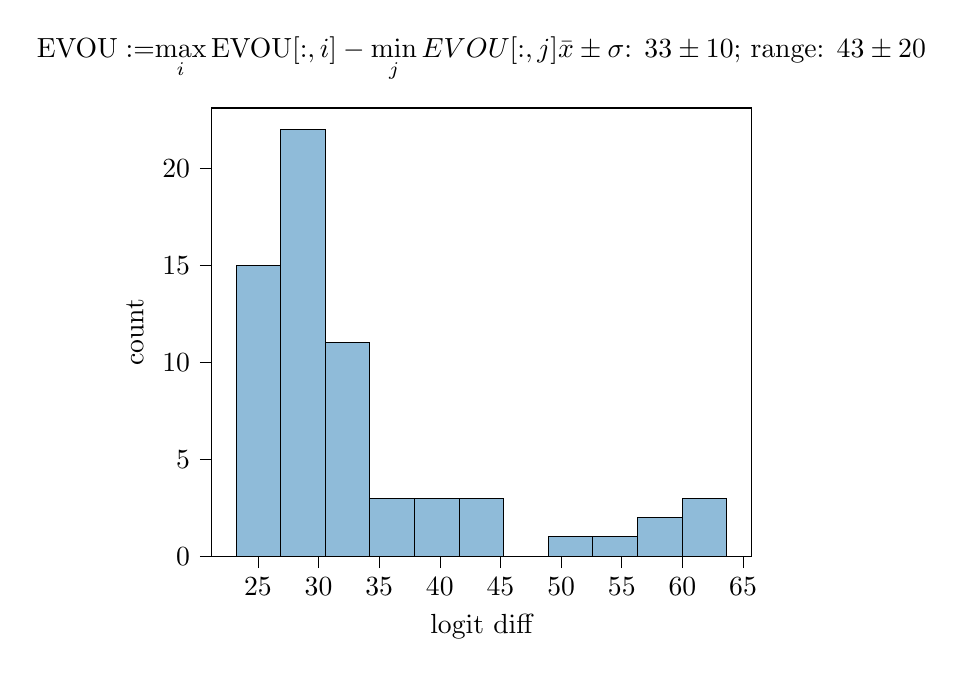
\begin{tikzpicture}

\definecolor{darkgray176}{RGB}{176,176,176}
\definecolor{steelblue31119180}{RGB}{31,119,180}

\begin{axis}[
tick align=outside,
tick pos=left,
title={\(\displaystyle \mathrm{EVOU} := \WE \WV \WO\WU \)\\
\(\displaystyle \max_i\mathrm{EVOU}[:,i] - \min_jEVOU[:,j]\)\\
\(\displaystyle \bar{x}\pm\sigma\): \(\displaystyle 33 \pm 10\); range: \(\displaystyle 43 \pm 20\)},
x grid style={darkgray176},
xlabel={logit diff},
xmin=21.1832078933716, xmax=65.6721578598022,
xtick style={color=black},
xtick={20,25,30,35,40,45,50,55,60,65,70},
xticklabels={
  \(\displaystyle {20}\),
  \(\displaystyle {25}\),
  \(\displaystyle {30}\),
  \(\displaystyle {35}\),
  \(\displaystyle {40}\),
  \(\displaystyle {45}\),
  \(\displaystyle {50}\),
  \(\displaystyle {55}\),
  \(\displaystyle {60}\),
  \(\displaystyle {65}\),
  \(\displaystyle {70}\)
},
y grid style={darkgray176},
ylabel={count},
ymin=0, ymax=23.1,
ytick style={color=black},
ytick={0,5,10,15,20,25},
yticklabels={
  \(\displaystyle {0}\),
  \(\displaystyle {5}\),
  \(\displaystyle {10}\),
  \(\displaystyle {15}\),
  \(\displaystyle {20}\),
  \(\displaystyle {25}\)
}
]
\draw[draw=black,fill=steelblue31119180,fill opacity=0.5] (axis cs:23.2054328918457,0) rectangle (axis cs:26.8822056163441,15);
\draw[draw=black,fill=steelblue31119180,fill opacity=0.5] (axis cs:26.8822056163441,0) rectangle (axis cs:30.5589783408425,22);
\draw[draw=black,fill=steelblue31119180,fill opacity=0.5] (axis cs:30.5589783408425,0) rectangle (axis cs:34.2357510653409,11);
\draw[draw=black,fill=steelblue31119180,fill opacity=0.5] (axis cs:34.2357510653409,0) rectangle (axis cs:37.9125237898393,3);
\draw[draw=black,fill=steelblue31119180,fill opacity=0.5] (axis cs:37.9125237898393,0) rectangle (axis cs:41.5892965143377,3);
\draw[draw=black,fill=steelblue31119180,fill opacity=0.5] (axis cs:41.5892965143377,0) rectangle (axis cs:45.2660692388361,3);
\draw[draw=black,fill=steelblue31119180,fill opacity=0.5] (axis cs:45.2660692388361,0) rectangle (axis cs:48.9428419633345,0);
\draw[draw=black,fill=steelblue31119180,fill opacity=0.5] (axis cs:48.9428419633345,0) rectangle (axis cs:52.6196146878329,1);
\draw[draw=black,fill=steelblue31119180,fill opacity=0.5] (axis cs:52.6196146878329,0) rectangle (axis cs:56.2963874123313,1);
\draw[draw=black,fill=steelblue31119180,fill opacity=0.5] (axis cs:56.2963874123313,0) rectangle (axis cs:59.9731601368297,2);
\draw[draw=black,fill=steelblue31119180,fill opacity=0.5] (axis cs:59.9731601368297,0) rectangle (axis cs:63.6499328613281,3);
\end{axis}

\end{tikzpicture}
